\documentclass{beamer}

\mode<presentation>
{
  \usetheme{CambridgeUS}      % or try Darmstadt, Madrid, ...
  \usecolortheme{default} % or try albatross, beaver, crane, ...
  \usefonttheme{default}  % or try serif, structurebold, ...
  \setbeamertemplate{navigation symbols}{}
  \setbeamertemplate{caption}[numbered]
} 

\usepackage[english]{babel}
\usepackage[utf8x]{inputenc}
\usepackage{listings}
\usepackage[ampersand]{easylist}



\definecolor{KTI_green}{RGB}{150, 189, 13}
\definecolor{TU_red}{RGB}{255, 55, 81}
\definecolor{faint_gray}{RGB}{180, 180, 180}

\definecolor{syntax_green}{rgb}{0,0.6,0}
\definecolor{syntax_gray}{rgb}{0.9, 0.9, 0.9}
\definecolor{syntax_mauve}{rgb}{0.58,0,0.82}

\lstset{ 
  backgroundcolor=\color{syntax_gray},  % choose the background color
  basicstyle=\scriptsize\ttfamily,        		% size of fonts used for the code
  breaklines=false,                		% automatic line breaking only at whitespace
  captionpos=b,                    		% sets the caption-position to bottom
  commentstyle=\color{syntax_green},    % comment style
  escapeinside={\%*}{*)},          		% if you want to add LaTeX within your code
  keywordstyle=\color{blue},       		% keyword style
  stringstyle=\color{syntax_mauve},     % string literal style
  columns=fullflexible,
  frame=single,
  framesep=0.5cm,
  framexleftmargin=0.5cm,
  xleftmargin=0.5cm,
  framexrightmargin=0.5cm,
  xrightmargin=0.5cm,
  frame=tb,                 
    numbers=left,                    
    numbersep=15pt,  
  }
  
  
\newcommand{\logopython}{\raggedleft 
\includegraphics[height=0.5cm]{logo_python}\hspace{0.1cm}\\\raggedright}
\newcommand{\logopythonbottom}{\raggedleft\vspace{-0.8cm}
\includegraphics[height=0.5cm]{logo_python}\hspace*{0.05cm}\\\raggedright}

\title[BSP24 - Garantiezertifikat]{Garantiezertifikat}
\author{Dickbauer Y., Moser P., Perner M.}
\institute{PS Computergestützte Modellierung, WS 2016/17}
%\date{Date of Presentation}

\begin{document}

\begin{frame}
  \titlepage
\end{frame}

\begin{frame}{Outline}
  \tableofcontents
\end{frame}

\section{Aufgabenstellung}
\begin{frame}{Aufgabenstellung}
Garantie-Zertifikate sichern entweder die Rückzahlung des gesamten oder eines bestimmten Prozentsatzes des eingesetzten Kapitals am Ende der Laufzeit zu. Zusätzlich wird der Anleger meist mit einer bestimmten Partizipationsrate am Kursanstieg des jeweiligen Basiswertes beteiligt. Alternativ ist eine Kuponzahlung möglich, die von der Entwicklung des Basiswertes abhängig ist.
\\~\\
Das folgende fiktive Garantiezertifikat ist mittels Simulation zu bewerten.
\end{frame}


\begin{frame}{Aufgabenstellung - 10 Titel}
\begin{itemize}
	\item Das Zertifikat läuft über 5 Jahre und umfasst 10 Titel, die in der untenstehenden Tabelle inklusive Volatilität zusammengefasst sind.
	\vspace{.2cm}
	\begin{center}
	\begin{tabular}{l|l}
	Alianz	 		& 35.2\% \\ 
	BMW 			& 27.6\% \\ 
	Canon 			& 29.3\% \\ 
	E.On			& 21.7\% \\ 
	France Telecom	& 27.6\% \\ 
	Hewlett Packard & 34.6\% \\ 
	ING Group 		& 31.4\% \\ 
	Intel 			& 32.3\% \\ 
	Lloyds 			& 23.4\% \\ 
	Microsoft		& 24.6\% \\  
	\end{tabular} 
	\end{center}
\end{itemize}
\end{frame}

\begin{frame}{Aufgabenstellung - Zeitverlauf 5 Jahre}
\begin{itemize}
	\item T = 0: das Zertifikat wird mit einem Aufschlag von 3\% ausgegeben. Alle Titel werden zu diesem Zeitpunkt mit 100\% bewertet.
	\item T = 1: garantierte 6\% Zinsen werden ausbezahlt
	\item T = 2: Koupon von 10.0\% p.a., wenn keine der im Basket enthaltenen Aktien gleich
oder unter 68\% ihres Anfangswertes notiert, oder 0.0\% p.a. andernfalls.
	\item T = 3: Koupon von 10.0\% p.a., wenn keine der im Basket enthaltenen Aktien gleich
oder unter 68\% ihres Anfangswertes notiert, oder 20.0\% p.a., wenn keine der im
Basket enthaltenen Aktien gleich oder unter 68\% ihres Anfangswertes notiert und
in der vorherigen Periode kein Kupon gezahlt worden ist, oder 0.0\% p.a. andernfalls.
\end{itemize}
\end{frame}

\begin{frame}{Aufgabenstellung - Zeitverlauf 5 Jahre}
\begin{itemize}
	\item T = 4: Koupon von 10.0\% p.a., wenn keine der im Basket enthaltenen Aktien gleich
oder unter 68\% ihres Anfangswertes notiert, oder 20.0\% p.a., wenn keine der im
Basket enthaltenen Aktien gleich oder unter 68\% ihres Anfangswertes notiert und
in der vorhergehenden Periode kein Kupon gezahlt worden ist, oder 30.0\% p.a., wenn
keine der im Basket enthaltenen Aktien gleich oder unter 68\% ihres Anfangswertes
notiert und in den beiden vorhergehenden Perioden kein Kupon gezahlt worden ist,
oder 0.0\% p.a. andernfalls.
\end{itemize}
\end{frame}

\begin{frame}{Aufgabenstellung - Zeitverlauf 5 Jahre}
\begin{itemize}
	\item T = 5: Koupon von 10.0\% p.a., wenn keine der im Basket enthaltenen Aktien gleich
oder unter 68\% ihres Anfangswertes notiert, oder 20.0\% p.a., wenn keine der im
Basket enthaltenen Aktien gleich oder unter 68\% ihres Anfangswertes notiert und
in der vorhergehenden Periode kein Kupon gezahlt worden ist, oder 30.0\% p.a., wenn
keine der im Basket enthaltenen Aktien gleich oder unter 68\% ihres Anfangswertes
notiert und in den beiden vorhergehenden Perioden kein Kupon gezahlt worden ist,
oder 40.0\% p.a., wenn keine der im Basket enthaltenen Aktien gleich oder unter 68\%
ihres Anfangswertes notiert und in den drei vorhergehenden Perioden kein Kupon
gezahlt worden ist, oder 0.0\% p.a. andernfalls.
\end{itemize}

\begin{itemize}
	\item T = 6: Bei Fälligkeit Rückzahlung zu 100\% des Nominalbetrages.
	\item Die jeweiligen Auszahlungen müssen mit dem risikofreien Zinssatz von 2\% abgezinst werden.
\end{itemize}
\end{frame}

\begin{frame}{Aufgabenstellung - Simulation Wertänderung}

Die Wertänderung des Titel kann über folgende Formel simuliert werden:
\begin{equation*}
	W_{t+1} = max\left \{ W_t \cdot e^{(rMarket - vola^2/2) \cdot time + vola \cdot N(0,1) \cdot \sqrt{time}} , 0\right \}
\end{equation*}
wobei
\begin{itemize}
	\item \textit{vola} für die oben angeführte Volatilität steht,
	\item \textit{rMarket} für den Marktzinssatz (Annahme von 3\%),
	\item \textit{time} für die Anzahl an Perioden, falls in einem Schritt über mehrere Perioden simuliert werden soll (in diesem Beispiel soll jeweils von einer Periode zur nächsten gewechselt werden),
	\item und $N(0,1)$ für eine normalverteilte (0,1) Zufallszahl
\end{itemize}
\end{frame}


\begin{frame}{Aufgabenstellung}
\begin{itemize}
  \item Eingabe: -
  \vspace{1cm}
  \item Output: Wertentwicklung der einzelnen Titel je Periode, Niedrigster Wert, Kouponzahlung je Periode, abgezinster Wert
\end{itemize}
\end{frame}

\section{Flow Chart}
\begin{frame}{Flow Chart}
	\centering
  	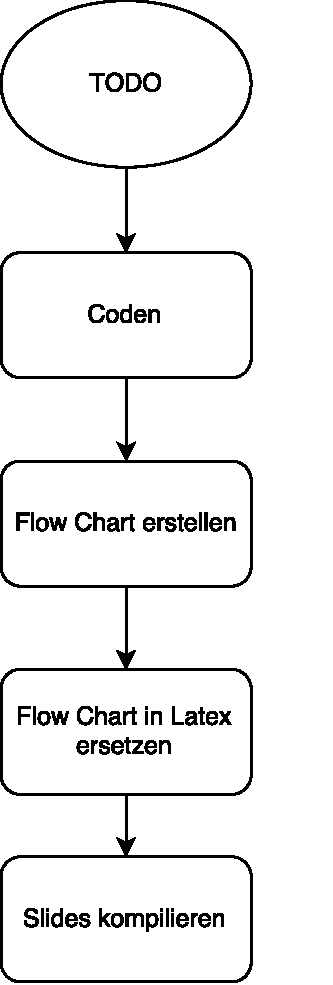
\includegraphics[scale=0.3]{FlowChartTodo.pdf}
\end{frame}

\subsection{Verwendete Funktionen}
%\begin{frame}[fragile]{Funktion loaded\_random\_choice(..)}
  \begin{itemize}
    \item Diese Funktion verlangt eine WSKL Liste als Eingabeparameter
    \item Gibt einen Index zurück, welcher 0 bis $\left\vert{probality\_list}\right\vert-1$ sein kann.
    \item Diese Indizes haben eine gewichtete WSKL, welche jeweils an der Position in der Eingabeliste steht
    \item Beispiel probility\_list := [ 0.9, 0.1 ]  $\Rightarrow$ mit p=90\% wird 0 zurückgegeben, p=10\% für 1
  \end{itemize}
  \begin{lstlisting}[language=python]
def loaded_random_choice(probability_list):
    n = len(probability_list)
    random_number = random.random()
    cum_p = 0
    for i in range(n):
        cum_p += probability_list[i]
        if cum_p > random_number:
            return i
    return None
\end{lstlisting}
\logopythonbottom
\end{frame}	

\section{Grafische Darstellung}

\end{document}
